\section{Continuous Relations by examples}

\marginnote{
\begin{rem}[Topological Space]
A \emph{topological space} is a pair $(X,\tau)$, where $X$ is a set, and $\tau \subset \mathcal{P}(X)$ are the \emph{open sets} of $X$, such that:
\begin{description}
    \item["nothing" and "everything" are open]  \[\varnothing,X \in \tau\]
    \item[Arbitrary unions of opens are open] \[\{ U_i : i \in I \} \subseteq \tau \Rightarrow \bigcup\limits_{i \in I} U_i \in \tau \]
    \item[Finite intersections of opens are open] $n \in \mathbb{N}$: \[U_1,\cdots, U_n \in \tau \Rightarrow \bigcap\limits_{1\cdots, i , \cdots n} U_i \in \tau\]
\end{description}
\end{rem}
}

\marginnote{
\begin{rem}[Relational Converse]
Recall that a relation $R: S \rightarrow T$ is a subset $R \subseteq S \times T$. \[R^\dag : T \rightarrow S := \{ (t,s) : (s,t) \in R \}\]
\end{rem}
}

\marginnote{
\begin{rem}[Continuous function]
A function between sets $f: X \rightarrow Y$ is a continuous function between topologies $f: (X,\tau) \rightarrow (Y,\sigma)$ if \[U \in \sigma \Rightarrow f^{-1}(U) \in \tau\] where $f^{-1}$ denotes the inverse image.
\end{rem}
}

\marginnote{
Recall that functions are relations, and the inverse image used in the definition of continuous maps is equivalent to the relational converse when functions are viewed as relations. So we can na\"{i}vely extend the notion of continuous maps to continuous relations between topological spaces.
}

\marginnote{
\begin{notation}
For shorthand, we denote the topology $(X,\tau)$ as $X^{\tau}$. As special cases, we denote the discrete topology on $X$ as $X^{\star}$, and the indiscrete topology $X^{\circ}$.
\end{notation}
}

\marginnote{
The symmetric monoidal structure is that of product topologies on objects, and products of relations on morphisms.
}

\marginnote{
\begin{rem}[Product Topology]
We denote the product topology of $X^\tau$ and $Y^\sigma$ as $(X \times Y)^{(\tau \times \sigma)}$. $\tau \times \sigma$ is the topology on $X \times Y$ generated by the basis $\{t \times s : t \in \mathfrak{b}_\tau, s \in \mathfrak{b}_\sigma\}$, where $\mathfrak{b}_\tau$ and $\mathfrak{b}_\sigma$ are bases for $\tau$ and $\sigma$ respectively.
\end{rem}
}

\marginnote{
\begin{rem}[Product of relations]
For relations between sets $R: X \rightarrow Y, S: A \rightarrow B$, the product relation $R \times S: X \times A \rightarrow Y \times B$ is defined to be \[ \{ ((x,a),(y,b)) : (x,y) \in R, (a,b) \in S \} \]
\end{rem}
}

\begin{defn}[Continuous Relation]\label{defn:Contrelation}
A continuous relation $R: (X,\tau) \rightarrow (Y,\sigma)$ is a relation $R: X \rightarrow Y$ such that \[U \in \sigma \Rightarrow R^{\dag}(U) \in \tau\] where $\dag$ denotes the relational converse.
\end{defn}

Let's consider three topological spaces and examine the continuous relations between them. This way we can build up intuitions, and prove some tool results in the process.

The \textbf{singleton space} consists of a single point which is both open and closed. We denote this space $\bullet$. Concretely, the underlying set and topology is
\[(\{\star\} \ , \ \{\{\star\},\varnothing\})\] 
\ctikzfig{testspaces/singleton}

The \textbf{Sierpi\'{n}ski space} consists of two points, one of which (in yellow) is open, and the other (in cyan) is closed. We denote this space $\mathcal{S}$. Concretely, the underlying set and topology is:
\[\big( \{0,1\} \ , \ \{ \varnothing, \{ 1 \} , \{ 0,1\} \} \big)\]
\ctikzfig{testspaces/sierpinski}

The \textbf{unit square} has $[0,1] \times [0,1]$ as its underlying set.  Open sets are "blobs" painted with open balls. Points, lines, and bounded shapes are closed. We denote this space $\blacksquare$.
\ctikzfig{testspaces/unitsquare}

\newthought{$\bullet \rightarrow \bullet$:} There are two relations from the singleton to the singleton; the identity relation $\{ (\bullet,\bullet) \}$, and the empty relation $\varnothing$. Both are topological.

\newthought{$\bullet \rightarrow \mathcal{S}$:} There are four relations from the singleton to the Sierpi\'{n}ski space, corresponding to the subsets of $\mathcal{S}$. All of them are topological.


\newthought{$\mathcal{S} \rightarrow \bullet$:}
\marginnote{
\begin{example}[A noncontinuous relation]\label{ex:nontop}
The relation $\{(0,\bullet)\} \subset \mathcal{S} \times \bullet$ is not a continuous relation: the preimage of the open set $\{\bullet\}$ under this relation is the non-open set $\{0\}$.
\end{example}
}
There four candidate relations from the Sierpi\'{n}ski space to the singleton, but as we see in Example \ref{ex:nontop}, not all of them are topological.

\newthought{Now we need some abstraction.} We cannot study the continuous relations between the singleton and the unit square case by case. We discover that continuous relations out of the singleton indicate arbitrary subsets, and that continuous relations into the singleton indicate arbitrary opens.
\marginnote{
\begin{term}
Call a continuous relation $\bullet \rightarrow X^\tau$ a \textbf{state} of $X^\tau$, and a continuous relation $X^\tau \rightarrow \bullet$ a \textbf{test} of $X^\tau$.
\end{term}

\begin{proposition}\label{prop:states}
States $R: \bullet \rightarrow X^{\tau}$ correspond with subsets of $X$.
\begin{proof}
The preimage $R^\dag(U)$ of a (non-$\varnothing$) open $U \in \tau$ is $\star$ if $R(\star) \cap U$ is nonempty, and $\varnothing$ otherwise. Both $\star$ and $\varnothing$ are open in $\{\star\}^{\bullet}$. $R(\star)$ is free to specify any non-$\varnothing$ subset of $X$. The empty relation handles $\varnothing$ as an open of $X^{\tau}$.
\end{proof}
\end{proposition}

\begin{proposition}\label{prop:tests}
Tests $R: X^\tau \rightarrow \bullet$ correspond with open sets $U \in \tau$.
\begin{proof}
The preimage $R^\dag(\star)$ of $\star$ must be an open set of $X^\tau$ by definition \ref{defn:toprelation}. $R^\dag(\star)$ is free to specify any open set of $X^{\tau}$.
\end{proof}
\end{proposition}
}

\newthought{$\bullet \rightarrow \blacksquare$:} Proposition \ref{prop:states} tells us that there are as many continuous relations from the singleton to the unit square as there are subsets of the unit square.

\newthought{$\blacksquare \rightarrow \bullet$:} Proposition \ref{prop:tests} tells us that there are as many continuous relations from the unit square to the singleton as there are open sets of the unit square.

\newthought{There are 16 candidate relations $\mathcal{S} \rightarrow \mathcal{S}$ to check.} A case-by-case approach won't scale, so we could instead identify the building blocks of continuous relations with the same source and target space.

\newthought{Given two continuous relations $R,S : X^\tau \rightarrow Y^\sigma$, how can we combine them?}\marginnote{
\begin{rem}[Union, intersection, and ordering of relations]
Recall that relations $X \rightarrow Y$ can be viewed as subsets of $X \times Y$. So it makes sense to speak of the union and intersection of relations, and of partially ordering them by inclusion.
\end{rem}
}

\begin{proposition}\label{prop:framehom}
If $R,S: X^\tau \rightarrow Y^\sigma$ are continuous relations, so are $R \cap S$ and $R \cup S$.
\begin{proof}
Replace $\square$ with either $\cup$ or $\cap$. For any non-$\varnothing$ open $U \in \sigma$: \[(R \square S)^\dag (U) = R^\dag(U) \square S^\dag(U)\] As $R,S$ are continuous relations, $R^\dag(U),S^\dag(U) \in \tau$, so $R^\dag(U) \square S^\dag(U) = (R \square S)^\dag (U) \in \tau$. Thus $R\square S$ is also a continuous relation.
\end{proof}
\end{proposition}

\begin{corollary}\label{cor:homspace}
Continuous relations $X^\tau \rightarrow Y^\sigma$ are closed under arbitrary union and finite intersection. Hence, continuous relations $X^\tau \rightarrow Y^\sigma$ form a topological space where each continuous relation is an open set on the base space $X \times Y$, where the full relation $X \rightarrow Y$ is "everything", and the empty relation is "nothing".
\end{corollary}

\newthought{A topological basis for spaces of continuous relations}
\marginnote{
\begin{rem}[Topological Basis]
$\mathfrak{b} \subseteq \tau$ is a basis of the topology $\tau$ if every $U \in \tau$ is expressible as a union of elements of $\mathfrak{b}$. Every topology has a basis (itself). Minimal bases are not necessarily unique.
\end{rem}
}

\begin{defn}[Partial Functions]
A \textbf{partial function} $X \rightarrow Y$ is a relation for which each $x \in X$ has at most a single element in its image. In particular, all functions are special cases of partial functions, as is the empty relation.
\end{defn}

\begin{lemma}[Partial functions are a $\cap$-ideal]\label{lem:capideal}
The intersection $f \cap R$ of a partial function $f: X \rightarrow Y$ with any other relation $R: X \rightarrow Y$ is again a partial function.
\begin{proof}
Consider an arbitrary $x \in X$. $R(x) \cap f(x) \subseteq f(x)$, so the image of $x$ under $f \cap R$ contains at most one element, since $f(x)$ contains at most one element.
\end{proof}
\end{lemma}

\begin{marginfigure}
\centering
\scalebox{0.5}{\tikzfig{paintingexamples/sierandcanvas2_2}}
\caption{Regions of $\blacksquare$ in the image of the yellow point alone will be coloured yellow, and regions in the image of both yellow and cyan will be coloured green:}
\label{fig:yellowgreen}
\end{marginfigure}

\begin{lemma}[Any single edge can be extended to a continuous partial function]\label{lem:edgecomplete}
Given any $(x,y) \in X \times Y$, there exists a continuous partial function $X^\tau \rightarrow Y^\sigma$ that contains $(x,y)$.
\begin{proof}
Let $\mathcal{N}(x)$ denote some open neighbourhood of $x$ with respect to the topology $\tau$. Then $\{ (z,y) : z \in \mathcal{N}(x) \}$ is a continuous partial function that contains $(x,y)$.
\end{proof}
\end{lemma}

\begin{marginfigure}
\centering
\scalebox{0.5}{\tikzfig{paintingexamples/s2sqzoom}}
\caption{Regions in the image of the cyan point alone cannot be open sets by continuity, so they are either points or lines. Points and lines in cyan must be surrounded by an open region in either yellow or green, or else we violate continuity (open sets in red).}
\label{fig:cyan}
\end{marginfigure}

\begin{marginfigure}
\centering
\scalebox{0.75}{\tikzfig{paintingexamples/s2sqpainting}}
\caption{A continuous relation $\mathcal{S} \rightarrow \blacksquare$: "Flower and critter in a sunny field".}
\label{fig:flower}
\end{marginfigure}

\begin{marginfigure}
\centering
\scalebox{0.75}{\tikzfig{paintingexamples/sq2spainting}}
\caption{A continuous relation $\blacksquare \rightarrow \mathcal{S}$: "still math?". Black lines and dots indicate gaps.}
\label{fig:shitpost}
\end{marginfigure}

\begin{proposition}\label{prop:hombasis}
Continuous partial functions form a topological basis for the space $(X \times Y)^{(\tau \multimap \sigma)}$, where the opens are continuous relations $X^\tau \rightarrow Y^\sigma$.
\begin{proof}
We will show that every continuous relation $R: X^\tau \rightarrow Y^\sigma$ arises as a union of continuous partial functions. Denote the set of continuous partial functions $\mathfrak{f}$. We claim that:
\[ R = \bigcup\limits_{F \in \mathfrak{f}} (R \cap F) \]
The $\supseteq$ direction is evident, while the $\subseteq$ direction follows from Lemma \ref{lem:edgecomplete}.
By Lemma \ref{lem:capideal}, every $R \cap F$ term is a partial function, and by Corollary \ref{cor:homspace}, continuous.
\end{proof}
\end{proposition}

\newthought{$\mathcal{S} \rightarrow \mathcal{S}$:} We can use Proposition \ref{prop:hombasis} to write out the topological basis of continuous partial functions, from which we can take unions to find all the continuous relations, which we depict in Figure \ref{fig:hassesierpinski}.

\newthought{$\mathcal{S} \rightarrow \blacksquare$:}
Now we use the colour convention of the points in $\mathcal{S}$ to "paint" continuous relations on the unit square "canvas", as in Figures \ref{fig:yellowgreen} and \ref{fig:cyan}. So each continuous relation is a painting, and we can characterise the paintings that correspond to continuous relations $\mathcal{S} \rightarrow \blacksquare$ in words as follows: Cyan only in points and lines, and either contained in or at the boundary of yellow or green. Have as much yellow and green as you like.

\newthought{$\blacksquare \rightarrow \mathcal{S}$:} The preimage of all of $\mathcal{S}$ must be an open set. So the painting cannot have stray lines or points outside of blobs. The preimage of yellow must be open, so the union of yellow and green in the painting cannot have stray lines or points outside of blobs. Point or line gaps within blobs are ok. Each connected blob can contain any colours in any shapes, subject to the constraint that if cyan appears anywhere, then either yellow or green must occur somewhere. Open blobs with no lines or points outside. Yellow and green considered alone is a painting made of blobs with no stray lines or points. If cyan appears anywhere, then either yellow or green have to appear somewhere.

\begin{figure}\label{fig:hassesierpinski}
\centering
\scalebox{0.5}{\tikzfig{testspaces/sierpinskienum}}
\caption{Hasse diagram of all continuous relations from the Sierpi\'{n}ski space to itself. Each relation is depicted left to right, and inclusion order is bottom-to-top. Relations that form the topological basis are boxed.}
\end{figure}

\clearpage

\newthought{One more example for fun: $[0,1] \rightarrow \blacksquare$:} We know how continuous functions from the unit line into the unit square look.
\begin{marginfigure}
\centering
\scalebox{0.5}{\tikzfig{paintingexamples/contline}}
\caption{
continuous functions $[0,1] \rightarrow \blacksquare$ follow the na\"{i}ve notion of continuity: a line one can draw on paper without lifting the pen off the page.
}
\label{fig:contline}
\end{marginfigure}
\newthought{Then what are the partial continuous functions?} If we understand these, we can obtain all continuous relations by arbitrary unions of the basis. Observe that the restriction of any continuous function to an open set in the source is a continuous partial function. The open sets of $[0,1]$ are collections of open intervals, each of which is homeomorphic to $(0,1)$, which is close enough to $[0,1]$.
%
\begin{marginfigure}
\centering
\scalebox{0.5}{\tikzfig{paintingexamples/contlines}}
\caption{
So a continuous partial function is \texttt{"(countably) many (open-ended) lines, each of which one can draw on paper without lifting the pen off the page."}
}
\label{fig:contline}
\end{marginfigure}
%
\begin{marginfigure}
\centering
\scalebox{0.5}{\tikzfig{paintingexamples/thickbrush}}
\caption{We can control the thickness of the brushstroke, by taking the union of (uncountably) many lines.}
\label{fig:thickbrush}
\end{marginfigure}

\newthought{Any painting is a continuous relation $[0,1] \rightarrow \blacksquare$.} By colour-coding $[0,1]$ and controlling brushstrokes, we can do quite a lot. Now we would like to develop the abstract machinery required to \emph{formally} paint pictures with words.

\begin{marginfigure}
\centering
\scalebox{0.8}{
\includegraphics{figures/paintingexamples/spectrum.png}}
\caption{Assign the visible spectrum of light to $[0,1]$. Colour open sets according to perceptual addition of light, computing brightness by normalising the measure of the open set.}
\end{marginfigure}

\begin{marginfigure}
\centering
\scalebox{0.8}{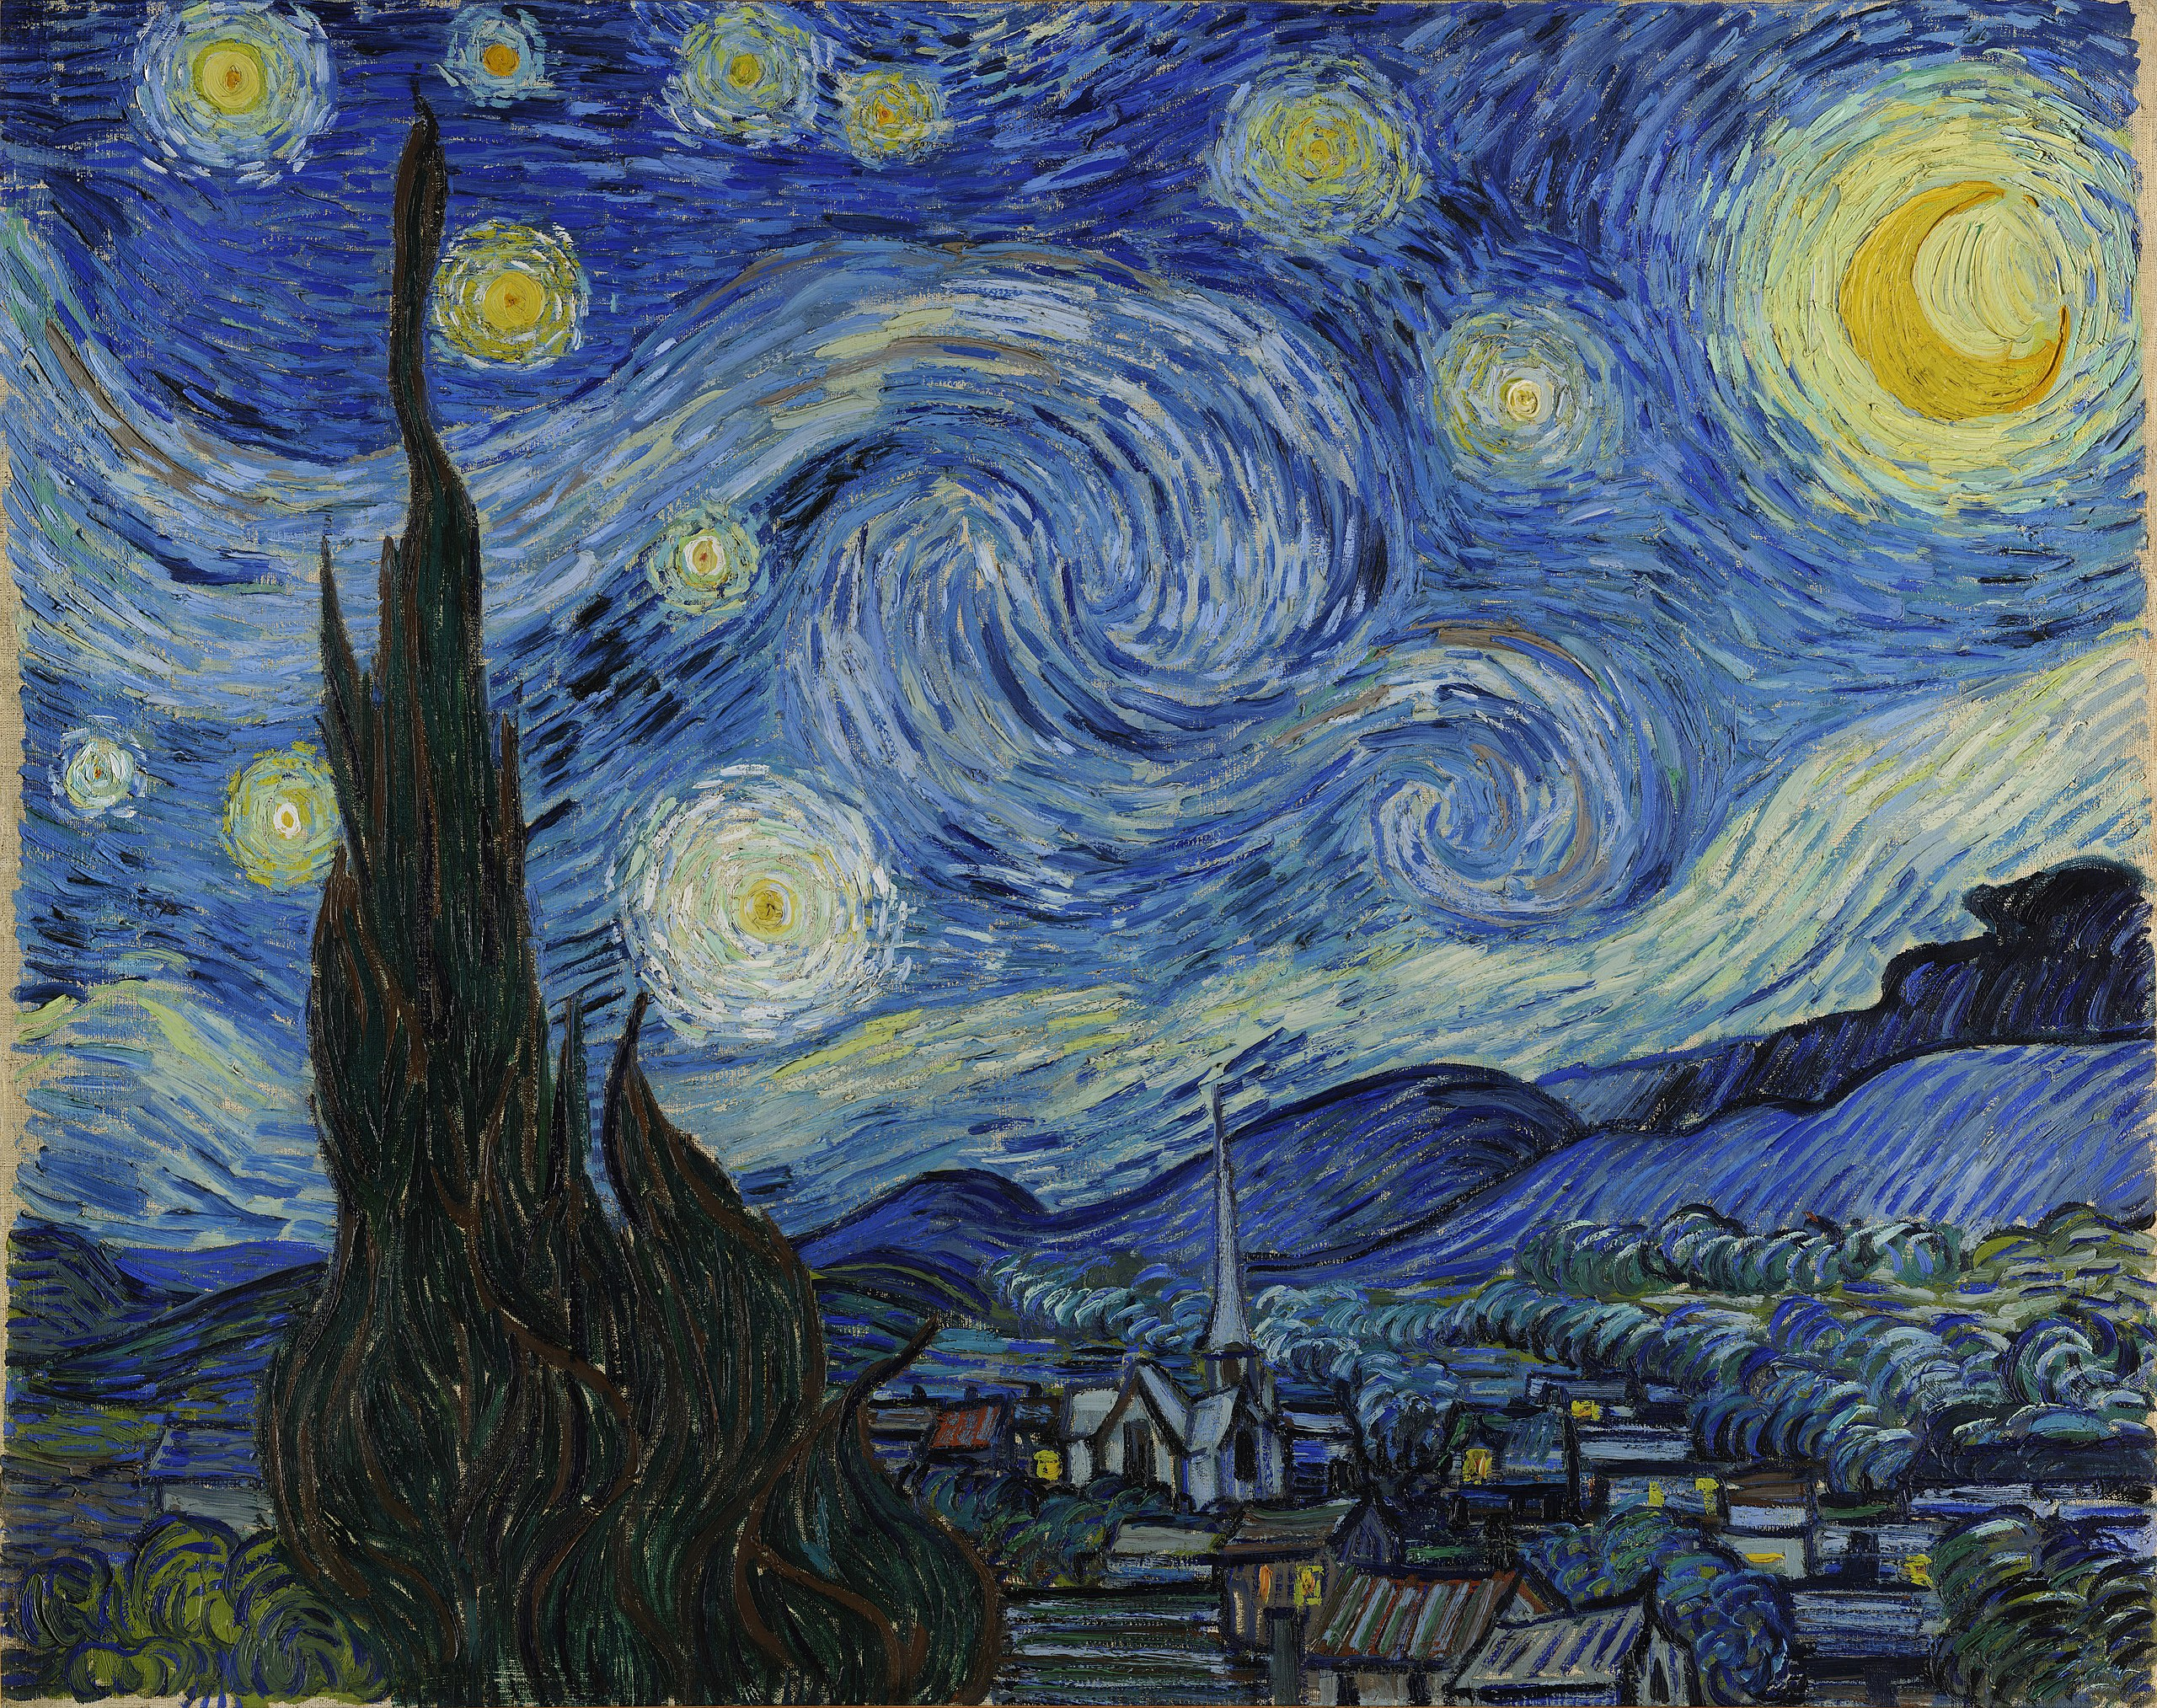
\includegraphics{figures/paintingexamples/starrynight}}
\caption{Like it or not, a continuous relation $[0,1] \rightarrow \blacksquare$: "The Starry Night", by Vincent van Gogh.}
\end{marginfigure}

\newthought{As one more step towards abstraction, we ask: which relations $X^\tau \rightarrow Y^\sigma$ are always continuous?}

\begin{proposition}
The \textbf{empty relation} $X \rightarrow Y$ relates nothing. It is defined $\varnothing \subset X \times Y$. The empty relation is always continuous.
\label{prop:emptyrel}
\begin{proof}
The preimage of the empty relation is always $\varnothing$, which is open by definition.
\end{proof}
\end{proposition}

\begin{proposition}\label{prop:fullrel}
The \textbf{full relation} $X \rightarrow Y$ relates everything to everything. It is all of $X \times Y$. Full relations are always continuous.
\begin{proof}
The preimage of any subset of $Y$ under the full relation is the whole of $X$, which is open by definition.
\end{proof}
\end{proposition}

\begin{proposition}\label{prop:bowtie}
Full relations restricted to open sets in the domain are continuous. Given an open $U \subseteq X^\tau$, and an arbitrary subset $K \subset Y^\sigma$, the relation $U \times K \subseteq X \times Y$ is open.
\begin{proof}
Consider an arbitrary open set $V \in \sigma$. Either $V$ and $K$ are disjoint, or they overlap. If they are disjoint, the preimage of $V$ is $\varnothing$, which is open. If they overlap, the preimage of $V$ is $U$, which is open.
\end{proof}
\end{proposition}

\begin{proposition}\label{prop:func}
Continuous functions are always continuous. If $f: X^\tau \rightarrow Y^\sigma$ is a continuous function, then it is also a continuous relation.
\begin{proof}
Functions are special cases of relations. The relational converse of a function viewed in this way is the same thing as the preimage.
\end{proof}
\end{proposition}

\begin{proposition}\label{prop:idrel}
The \textbf{identity relation} $X \rightarrow X$ relates anything to itself. It is defined $\{(x,x) : x \in X\} \subseteq X \times X$. The identity relation is always continuous.
\begin{proof}
The preimage of any open set under the identity relation is itself, which is open by assumption. The identity relation is also the "trivial" continuous map from a space to itself, so this also follows from Proposition \ref{prop:func}.
\end{proof}
\end{proposition}